\documentclass{article}

% if you need to pass options to natbib, use, e.g.:
%     \PassOptionsToPackage{numbers, compress}{natbib}
% before loading neurips_2021

% ready for submission
\usepackage{neurips_2021}
\usepackage{graphicx}
\usepackage{dsfont}

% IMPORTANT: if you are submitting attention track, please add the attention option:
% \usepackage[attention]{neurips_2021}

% to compile a preprint version, e.g., for submission to arXiv, add add the
% [preprint] option:
%     \usepackage[preprint]{neurips_2021}

% to compile a camera-ready version, add the [final] option, e.g.:
%     \usepackage[final]{neurips_2021}

% to avoid loading the natbib package, add option nonatbib:
%    \usepackage[nonatbib]{neurips_2021}

\usepackage[utf8]{inputenc} % allow utf-8 input
\usepackage[T1]{fontenc}    % use 8-bit T1 fonts
\usepackage{hyperref}       % hyperlinks
\usepackage{url}            % simple URL typesetting
\usepackage{booktabs}       % professional-quality tables
\usepackage{amsfonts}       % blackboard math symbols
\usepackage{nicefrac}       % compact symbols for 1/2, etc.
\usepackage{microtype}      % microtypography
\usepackage{xcolor}         % colors
\bibliographystyle{unsrtnat}

\title{Automated Protein Function Description for Novel Class Discovery}

% The \author macro works with any number of authors. There are two commands
% used to separate the names and addresses of multiple authors: \And and \AND.
%
% Using \And between authors leaves it to LaTeX to determine where to break the
% lines. Using \AND forces a line break at that point. So, if LaTeX puts 3 of 4
% authors names on the first line, and the last on the second line, try using
% \AND instead of \And before the third author name.

\author{Meet Barot \\
        Center for Data Science, New York University\\
		60 5th Avenue\\
        New York, NY 10011\\
        \texttt{meetbarot@nyu.edu}
  % examples of more authors
  \And
  Vladimir Gligorijevic\\
  Prescient Design, Genentech\\
  149 5th Avenue\\
  \texttt{gligorijevic.vladimir@gene.com} \\
  \AND
  Richard Bonneau \\
  Prescient Design, Genentech\\
  New York University Biology \\
  149 5th Avenue\\
  \texttt{bonneau.richard@gene.com} \\
  \And
  Kyunghyun Cho \\
  Courant Institute and Center for Data Science, New York University \\
  60 5th Avenue \\
  New York, NY 10011\\
  \texttt{kyunghyun.cho@nyu.edu} \\
}

\begin{document}

\maketitle

\begin{abstract}
Knowledge of protein function is necessary for understanding biological systems, but the discovery of new sequences from high-throughput sequencing technologies far outpaces their functional characterization.
Beyond the problem of assigning newly sequenced proteins to known functions, a more challenging issue is discovering novel protein functions.
The space of possible functions becomes unlimited when considering designed proteins.
Protein function prediction, as it is framed in the case of Gene Ontology term prediction, is a multilabel problem with a hierarchical label space.
However, this framing is limiting. It does not provide guiding principles for discovering completely novel functions.
In this work we propose a neural machine translation model in order to generate descriptions of protein functions in natural language.
We design metrics to evaluate different aspects of model performance: correctness, specificity and robustness. 
We provide results of our model in the zero-shot classification setting, scoring functional descriptions that the model has not seen before for proteins that have limited homology to those in the training set. 
Finally, we show generated function descriptions compared to ground truth descriptions for qualitative evaluation.
\end{abstract}

\section{Introduction}

    Determining the function of proteins is a fundamental problem in biology.
    Accurately identifying these functions through wetlab experimentation is costly, so computational approaches to predict protein function have been necessary to reduce the functional search space for experimentalists.
    However, many existing approaches to protein function prediction are only able to predict known functional categories, leaving out the possibility of classifying proteins into new categories.

    In this work, we propose a framing of the protein function prediction problem that does not rely on discrete categories. 
    Instead, we directly predict the common functional description of a group of proteins in natural language, modeling the problem as a neural machine translation task. 
    We train our model on about 300k protein sequences from the Swiss-Prot database \citep{SwissProt} annotated with functional descriptions from the Gene Ontology (GO) \citep{GO}.
    We show that the model is capable of generating accurate function descriptions of proteins that are less than 30\% identical to sequences in the training set and that have functions not present in the training set.
    We also propose three metrics to evaluate the correctness, specificity, and robustness of any model that can assign probabilities to a given sequence set and description.

    \section{Related Work}
    \subsection{Protein Function Prediction} 
    Many methods have been proposed for protein function prediction, though most do not consider the problem of discovering novel functions or generating their descriptions.
	As observed by \cite{friedberg2006automated}, this has mainly been because of inherent difficulties of the flexibility of natural language, such as synonymous terms and ambiguity. 
    These same difficulties were what led to the development of controlled and well-defined vocabularies of protein function, such as the Enzyme Commission Classification \citep{webb1992enzyme} and the Gene Ontology.
    As a result, the protein function prediction problem is generally framed as a supervised or semi-supervised multilabel problem with a structured output defined by these vocabularies, where the predicted labels are assumed to have some example in the training set \citep{bonetta2020machine}.
    Much focus has been placed on this framing. 
	The Critical Assessment of Functional Annotation \citep{CAFA3} serves as the main community benchmark for protein function prediction, and drives the field to improve upon previous methods.
	%The community submits new methods to annotate unlabeled proteins whose functional annotations are held out. 
	The CAFA evaluation datasets consider proteins that can described by existing categories, yet many unlabeled proteins, especially in understudied organisms, are likely to perform functions that have not been seen before.
    The supervised approach does not address this possibility, and so new methods must be proposed for function discovery.
	\subsection{Clustering}
    Flat clustering-based approaches, by themselves, are not able to give much information about the new functional categories that they predict.
    They can only predict that a protein may belong to a category that has not been studied.
    One could compute average distances to clusters that contain known proteins, but beyond this, there is no testable hypothesis that the model can give about their function.
    NeXO \citep{NeXO} and CliXO \citep{CliXO} are both methods that generate an ontology of protein functions given relationships between proteins using hierarchical clustering. They aim at discovering novel functions. 
	However, information about those new functions still rely on comparing the groupings to existing ontologies such as GO. 
    \cite{wang2018annotating} describe a method that creates a concept hierarchy from phrases automatically extracted from scientific literature. This concept hierarchy is then aligned with the CliXO ontology in order to annotate proteins. However, this approach is still less flexible than generating free-form natural language.
	\subsection{Zero-shot learning approaches}
    Zero-shot learning approaches attempt to address the unseen class problem directly.
    DeepGOZero \citep{DeepGOZero} is a method that uses ontology axioms to predict for classes with no examples in the training set.
    However, the classes that are able to be predicted must be defined with ontological relations to seen classes. 
	A similar limitation applies to clusDCA \citep{clusDCA}, which uses ontology relations to embed GO terms into a low dimensional space to perform zero-shot classification.

    This constraint both restricts the possible novel functions that can be discovered and may not give sufficient information to design an experiment to test for the novel function.

    \subsection{Text generation and neural machine translation}
    Neural network-based text generation approaches have made significant progress in generating fluent and meaningful text \citep{fatima2022systematic}. 
    Further, deep learning-based techniques have shown promising results in image captioning methods \citep{hossain2019comprehensive} and zero-shot classification of images\cite{CLIP}.
    Given enough data, deep learning methods have been shown to be capable of mapping between a range of input modalities and natural language.
    So far, there have been a few attempts to apply these methods to the protein function prediction domain.
    \cite{zhang2020automatic} use a graph-based generative model to generate Gene Ontology term names. However, the generation is limited to short phrases and relies on text descriptions from the GeneCards database \cite{GeneCards} for the input.

    Neural machine translation (NMT) is the automatic translation of written text from one natural language to another directly using neural networks \cite{cho2014properties}. NMT models have been widely deployed in production translation systems and show promise in domains other than natural language.
    Recently, a method called ProTranslator \citep{ProTranslator} has been proposed, which uses sequence, network and text description information concatenated into a 1-D feature vector in order to perform zero-shot classification on Gene Ontology terms.
    The authors also show that they are able to generate accurate and detailed descriptions for a set of proteins using a separate transformer model with this feature representation.
    Compared to ProTranslator, our method does not use any additional information to produce descriptions besides a set of protein sequences, and our model is trained directly to generate descriptions without pooling and losing positional information over the input sequences.

\section{Methods}
\begin{figure}
    \centering
    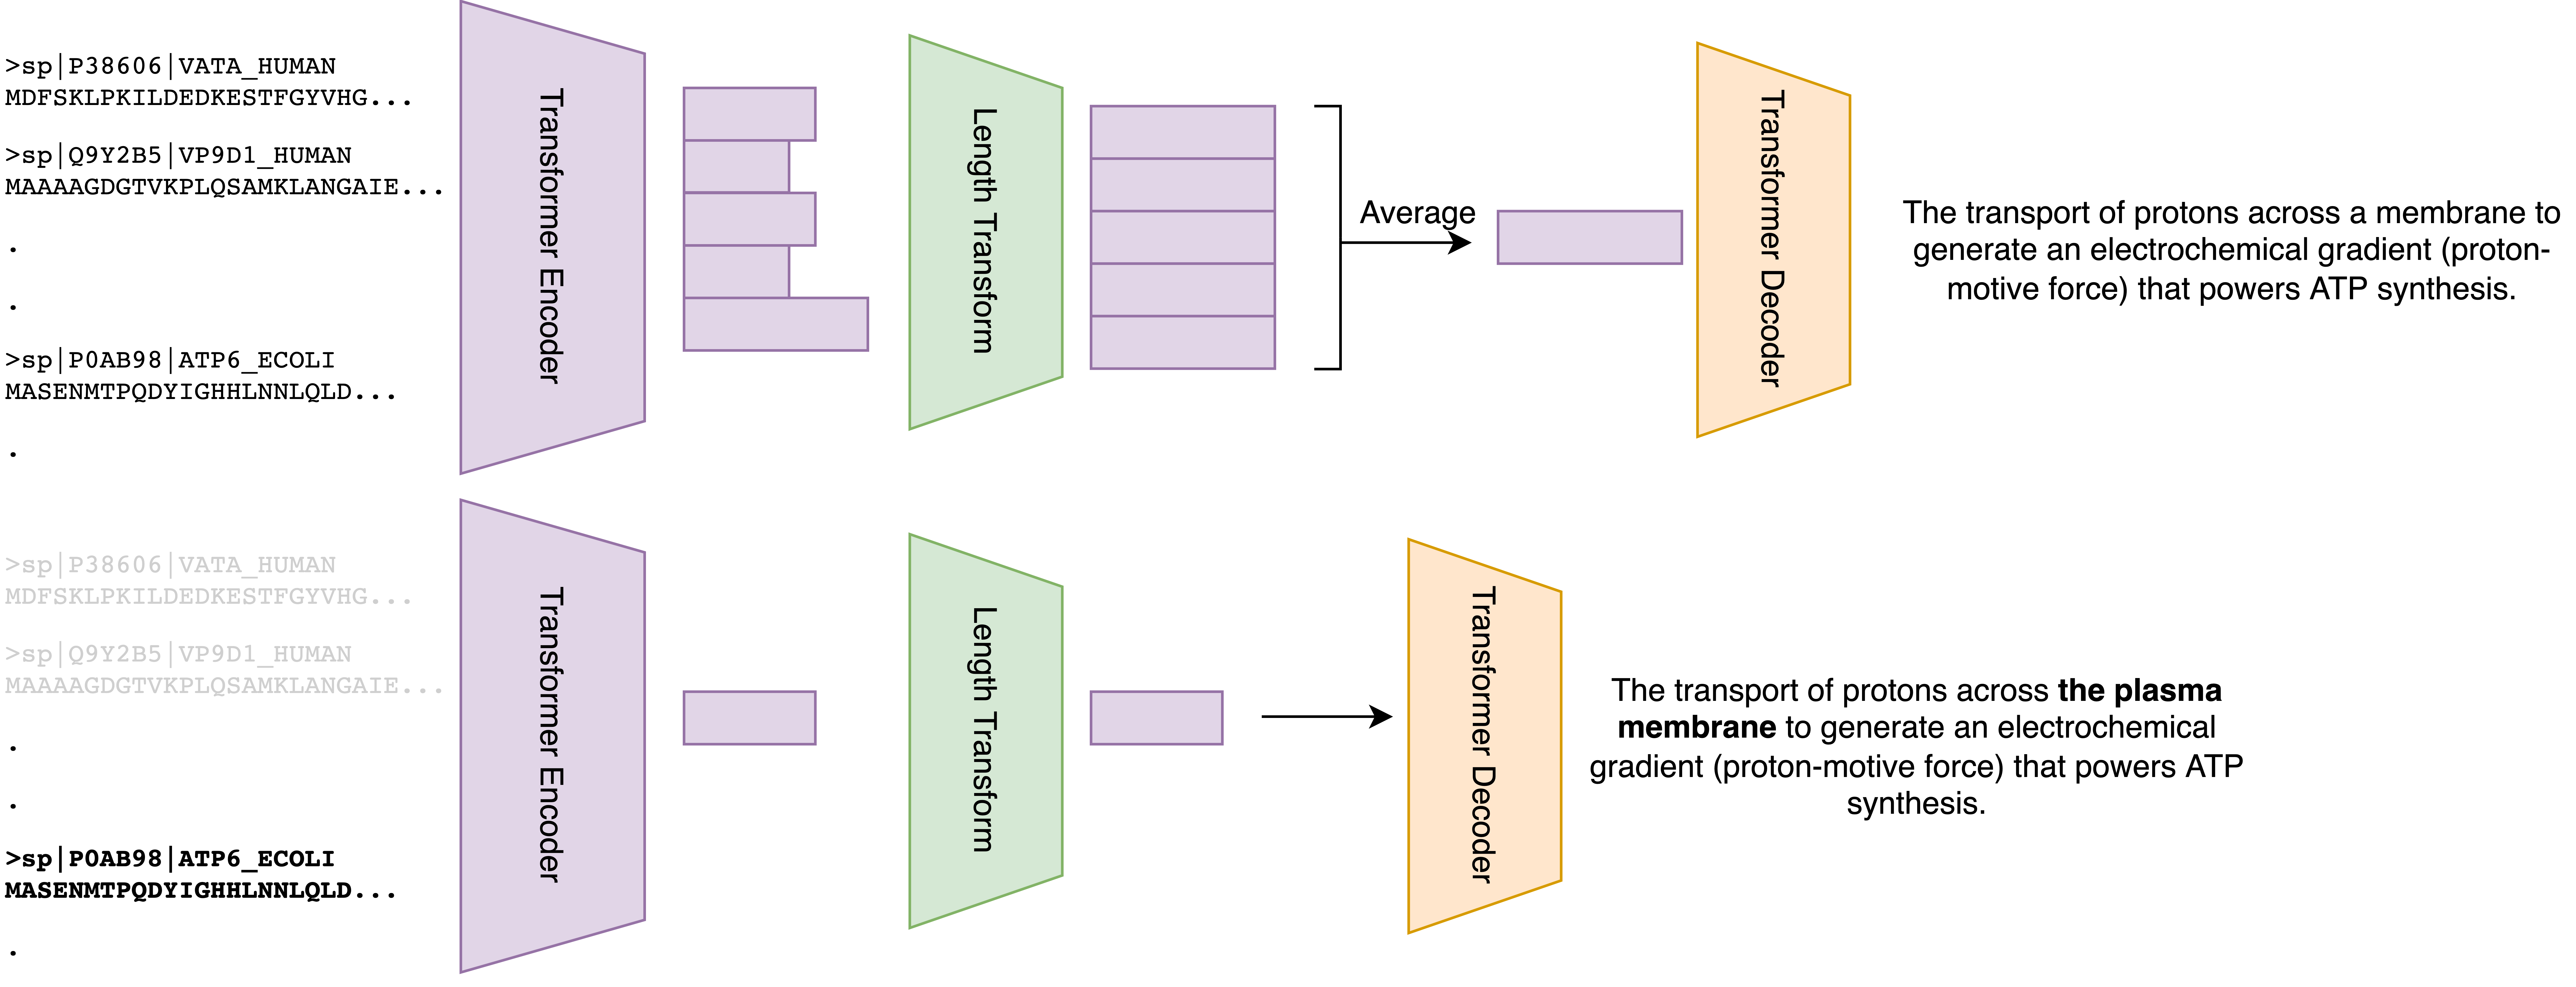
\includegraphics[width=0.9\linewidth]{prot2go.png}
    \caption{High-level diagram of the proposed transformer encoder-decoder model.
The model is trained to produce the most specific common function of the input protein sequences.}
    \label{overview}
\end{figure}
The following subsections give the motivation and formulations of the components of our method. Figure \ref{overview} contains a high-level overview.

        %Explicitly ontology-based zero-shot approaches such as DeepGOZero \citep{DeepGOZero} and clusDCA \cite{clusDCA} do not allow for actual description of a new function that is discovered.
        %    The only information that is gained is that the protein has a new function that has some specified ontological relation to currently known functions.
        %    However, this may not sufficiently describe the new function, and it also excludes possible functions that do not directly relate to known functions.
        %    In order to discover new categories of protein function, not dependent on existing categories, and with some amount of information to experimentally validate them, a model should ideally generate functional descriptions in natural language.
    
    \subsection{Protein sets to describe}
    %Let us consider a set of proteins $S$. Our goal is to find the most specific functional description $d_{S}^*$ that is common to all proteins in $S$. 
    %Protein functions are abstractions of what we know groups of proteins to do.  
    %Having a set of sequences as input is a more general framing that matches the way the GO terms themselves were created. % back this statement up a bit, probably from GO paper
    Biologists describe and categorize functions as abstractions of the common activity of a group of proteins, so we want our model to be able to perform this abstraction in a similar way.
    Formulating the problem as finding a single functional description for a single protein at a time is ill-defined, since a protein may have more than one function \cite{jeffery2018protein}.
    Let us consider a set of protein sequences $s \in S$, invariant to ordering, as input to our model.
    Our task, then, is to find a description $d_{S}$ which corresponds to the most specific function that is common to all protein sequences $s \in S$.

    \subsection{Transformer encoder-decoder model with length transform}
    We use a transformer encoder-decoder model \citep{vaswani2017attention} with a length transform to handle differing sequence lengths in order to average sequence features from the encoder. 
    The sequences' representations should be combined in some way that preserves the amino acid ordering, so we use the length transform in order to shape the representations such that they can be combined while order information is preserved.
    For each sequence $s \in S$, we use a transformer model with positional encoding and self-attention to obtain a representation $h_{s}$ which consists of $|s|$ continuous-valued vectors. 
    As described in \cite{shu2020latent}, the length transform takes the input $h_{s}$ of length $|s|$ and transforms the sequence with a monotonic location-based attention into a representation $h^{max}_{s}$ such that $|h^{max}_{s}| = max_{s \in S}|s|$. 
    
    \subsection{Autoregressive generation of descriptions}
    It is desirable to represent protein function in a compositional way, so that the model has the ability to describe any given set of proteins. To do this, we generate protein function descriptions in natural language, which gives the model the capability to describe a new function rather than having to rely on training examples of that function. We predict the tokens autoregressively, which is a standard practice in the NMT literature of top performing methods.
    With the $|S|$ sequence representations $h^{max}_{s}$ having all the same length after the length transform, we are able to take the average of these abstract representations, giving us $h_{S}$, the representation of the sequence set. We use this representation in the transformer decoder in order to predict the next token of the description given all the previous tokens.

    \subsection{Zero-shot Classification setting}
Fundamentally, our model assigns probabilities to pairs of protein sets and descriptions. In order to evaluate the method, we use the zero-shot classification setting, where we wish to classify proteins into unseen categories. We develop three metrics in the Evaluation section to evaluate the conditional probability distribution $P(d_{S}|S)$ learned by the model in this classification setting.

    \subsection{Generation (beam search)}
    Generation of descriptions is a search problem through the set of all possible output token sequences, where the goal is to find the sequence with the largest probability. Generation given an autoregressive model is a highly studied problem in the natural language processing literature.
    We use beam search \cite{graves2012sequence} in the current implementation in order to find reasonable generated descriptions. We use a beam width of 25 with a length penalty of 1.0. Direct evaluation of these descriptions is an unsolved problem: currently, manual inspection by expert human evaluators is the best method we have.

\section{Evaluation}
In this section, we define three metrics that can be computed using known functional descriptions in order to evaluate our models' learned probability distributions.

Generated descriptions are shown in the Results section for qualitative analysis.
Quantitative analysis of the generated descriptions requires data from human evaluators with expertise in protein function in order to determine the accuracy of generated descriptions.
A framework for performing that analysis with expert curators is explored in the Discussion section.
        \subsection{Attribute 1: Annotation correctness.}

        Given a sequence set for which the model is assigning scores to function descriptions, descriptions of GO terms that annotate the entire sequence set should be scored higher than terms that do not annotate the entire sequence set.

        Let $D_{S}$ be the GO term descriptions associated with sequence set S.

        \[P(d \in D_{S} | S) > P(d \notin D_{S} | S)\]

        A way to measure this attribute would be to calculate:
        \[\frac{1}{|D_{S}|*|D_{S}^{c}|}\sum_{d_i \in D_{S}, d_j \notin D_{S}} \mathds{1}(P(d_i | S) > P(d_j | S))\]
        where $D_{S}^{c}$ is the complement of $D_{S}$ and $\mathds{1}$ is the indicator function.

        \subsection{Attribute 2: Specificity preference.}

        Among terms that do annotate the whole set, the model should score child terms higher than their ancestor terms.
Let $A(d)$ denote the description of a direct parent of the GO term described by $d$.

        \[P(d \in D_{S}| S) > P(A(d) \in D_{S}| S)\]
        Note: any protein set that is annotated with $d$ would always be annotated with $A(d)$, $A(A((d))$ and so on.

        A way to measure this attribute would be to calculate:
        \[\frac{1}{|D_{S}|}\sum_{d_i \in D_{S}} \mathds{1}(P(d_i | S) > P(A(d_i) | S))\]

        \subsection{Attribute 3: Annotation robustness.}

        Any set of sequences that have the same exact set of GO descriptions in common should be scored with the same rankings for those GO descriptions.

        Let $S_i$ and $S_j$ be different sequence sets such that $D_{S_i} = D_{S_j}$ and $S_i \neq S_j$, and let $R(X)$ be a ranking function that gives the ranks of entries in $X$, in descending order.

        \[R_{d}(P(d \in D_{S_i} | S_i)) = R_{d}(P(d \in D_{S_i} | S_j))\]

        A way to measure this attribute would be to calculate the average Spearman's rank correlation of the rankings for all sequence sets' correct descriptions.
Let $R_{S_i} = R(P(D_{S_i} | S_i))$:

        \[\frac{1}{N*(N-1)}\sum_{S_i, S_j} \frac{\textnormal{cov}(R_{S_i}, R_{S_j})}{\sigma_{R_{S_i}}\sigma_{R_{S_j}}}\]

        where $N$ is the total number of sequence sets that have the exact set of GO descriptions $D_{S_i}$.
In reality, this number may be too large to actually sum (especially if $|D_{S_i}|$ is small), so we approximate this measure by subsampling $n < N$ sequence sets to average over instead.
The sum is only calculated over non-identical pairs of sequence sets.

\section{Data}
We take sequences and annotations from the Uniprot-KB Swiss-Prot database, which is manually annotated and reviewed, in order to create our training and evaluation sets of proteins and function descriptions. 
This database had 566,996 proteins total. 
To show that our model can generalize to non-homologous proteins, we clustered the proteins into groupings with less than 30\% sequence identity, and separated these into training and test sets. 
To focus on the functions that were both specific enough and had a sufficient number of examples in our evaluation sets, we restricted the maximum number of proteins per GO term to 1280, and minimum number of proteins to 32. 
Hyperparameters chosen were tuned on the training set proteins with training function descriptions.
The number of proteins and GO terms that were used after these restrictions in our training set and evaluation sets are listed in Table \ref{tab:datasets}.
\begin{table}
    \caption{Number of proteins and GO terms in training and test sets.}
	\centering
	\begin{tabular}{c|cccc}
		\toprule
         & Train P\&F & Train P, Test F & Test P, Train F & Test P\&F \\
		\midrule
        Prots & 316k & 181k & 20k & 20k \\
        Funcs & 9k & 2k & 879 & 1.5k \\
		\bottomrule
	\end{tabular}
	\label{tab:datasets}
\end{table}

\section{Results} % Need to see the naive performances that Kyungyhun suggested to compare to

        We show model performances in Table \ref{tab:performances}. The table suggests that the model is able to rank unseen functions for protein sets that it has been exposed to in training, with the model's rankings of identically annotated sets being in moderate agreement. For test proteins that have less than 30\% sequence identity to the training set, the model is still able to assign rankings of 1000 randomly selected functions from the training set with a correctness 30\% above random assignment (0.5). For the low-similarity test proteins that have functions that are not seen in the training set, the model is still able to rank 21\% better than random rankings.

        We are mainly focused on using the model for generation, and these metrics are meant mostly as guides for model design. The loss function used is not optimizing for classification accuracy; it is optimizing the model's probability distribution to assign high probability to descriptions assigned to a sequence set.

        We show sample test set descriptions in Table \ref{tab:descriptions}. The first row shows that the model describes verbatim a related term (GO:0001654, eye development) for the proteins selected, whereas the true term is appendage development (GO:0048736). Their common ancestor term is anatomical structure development (GO:0048856). This description is more specific than the actual term from which the proteins are sampled, but it is not accurate. The next generated description is more general than the actual description of the sampled set (modulates vs. activates), but is correct; it is the direct parent of the true term. The third generated description is related but ultimately different than the actual description of the protein set. The fourth generated description is more specific than both the true common GO description of the set (protein import, GO:0017038) and the generated description's closest known GO term, protein exit from endoplasmic reticulum (GO:0032527). It is describing protein import into the nucleus from the endoplasmic reticulum, which is not currently a GO term, but if it was, it would be a descendant of both of these terms.
\begin{table}
	\caption{Model Performances}
	\centering
	\begin{tabular}{l|llll}
		\toprule
        Metric & Train P, Test F & Test P, Train F & Test P\&F \\
		\midrule
        Annotation Correctness & 0.8844 & 0.8014 & 0.7157 \\
        Specificity Preference & 0.5765 & 0.5526 & 0.5701 \\
		Annotation Robustness & 0.4020 & 0.1977 & 0.2362 \\
		\bottomrule
	\end{tabular}
	\label{tab:performances}
\end{table}
\begin{table}
	\caption{Sample Test Set Description Generations}
	\centering
    \begin{tabular}{p{2 cm}|p{5 cm}|p{5 cm}|p{2 cm}}
		\toprule
        True Common GO Term & True Common GO Description of Sequence Set & Model Generated Description of Sequence Set & Closest Known GO Term to Generated Description\\
		\midrule
        GO:0048736, appendage development & <SOS> the process in which the anatomical structures of appendages are generated and organized . an appendage is an organ or part that is attached to the trunk of an organism . <EOS> & <SOS> the process whose specific outcome is the progression of the eye over time , from its formation to the mature structure . <EOS> & GO:0001654, eye development \\ \hline
        GO:0045597, positive regulation of cell differentiation & <SOS> any process that activates or increases the frequency , rate or extent of cell differentiation . <EOS> & <SOS> any process that modulates the frequency , rate or extent of cell differentiation . <EOS> & GO:0045595, regulation of cell differentiation  \\ \hline
        GO:0071162, CMG complex & <SOS> a protein complex that contains the gins complex , cdc45p , and the heterohexameric mcm complex , and that is involved in unwinding dna during replication . <EOS> & <SOS> any process involved in forming the mature 3 ' end of a dna ( mrna ) molecule . <EOS> & GO:0031124, mRNA 3'-end processing \\
        \hline
        GO:0017038, protein import & <SOS> the targeting and directed movement of proteins into a cell or organelle . not all import involves an initial targeting event . <EOS> & <SOS> the directed movement of proteins from endoplasmic reticulum to the nucleus . <EOS> & GO:0032527, protein exit from endoplasmic reticulum \\
		\bottomrule
	\end{tabular}
    \label{tab:descriptions}
\end{table}

\section{Discussion}
In this work, we have proposed a novel method to generate protein function descriptions in order to discover new protein functions.
We have demonstrated that our model can accurately rank unseen function descriptions for proteins not seen in the training set, and show promising results in generated function descriptions.
Below, we explore how we might further evaluate the method's generated descriptions using human expertise and curation.

\subsection{Future human-assisted evaluation of function discovery}
As our scoring metrics for evaluation are automated, they can be used for optimizing the architecture and other hyperparameters of the model (either manually or with some search method).
However, in the case of actual use on proteins that are not very well studied, it can be difficult to know whether a given description is accurate.
Human-assisted evaluation will be needed for the descriptions generated for a given set of novel proteins.
This feedback could be used to fine-tune the model to produce more accurate, fluid or generally desirable descriptions of proteins, as has been done for document summarization models \citep{finetuningWithHuman, learningToSummarize}.

One possible way of obtaining human feedback would be to ask an expert with knowledge of the Gene Ontology and familiarity with some families of proteins to choose between two descriptions for a given sequence set that is generated from a trained model.
Doing this over a large enough dataset would allow us to train a reward estimation model that can then be used to fine-tune the original trained model using reinforcement learning.
However, this would be expensive, as the task needs to be done by an expert.
Richer information, such as ranking the similarities to an existing GO term, or suggesting changes to particular portions of the description, could be used to increase performance even with a small number of examples with human feedback.


%\section{Submission of papers to NeurIPS 2021 AI for Science Workshop}
%
%Please read the instructions below carefully and follow them faithfully.
%
%\subsection{Style}
%
%Papers to be submitted to NeurIPS 2021 must be prepared according to the
%instructions presented here. Papers may only be up to {\bf nine} pages long,
%including figures. Additional pages \emph{containing only acknowledgments and
%references} are allowed. Papers that exceed the page limit will not be
%reviewed, or in any other way considered for presentation at the conference.
%
%The margins in 2021 are the same as those in 2007, which allow for $\sim$$15\%$
%more words in the paper compared to earlier years.
%
%Authors are required to use the NeurIPS \LaTeX{} style files obtainable at the
%NeurIPS website as indicated below. Please make sure you use the current files
%and not previous versions. Tweaking the style files may be grounds for
%rejection.
%
%\subsection{Retrieval of style files}
%
%The style files for NeurIPS and other conference information are available on
%the World Wide Web at
%\begin{center}
%  \url{http://www.neurips.cc/}
%\end{center}
%The file \verb+neurips_2021.pdf+ contains these instructions and illustrates the
%various formatting requirements your NeurIPS paper must satisfy.
%
%The only supported style file for NeurIPS 2021 is \verb+neurips_2021.sty+,
%rewritten for \LaTeXe{}.  \textbf{Previous style files for \LaTeX{} 2.09,
%  Microsoft Word, and RTF are no longer supported!}
%
%The \LaTeX{} style file contains three optional arguments: \verb+final+, which
%creates a camera-ready copy, \verb+preprint+, which creates a preprint for
%submission to, e.g., arXiv, and \verb+nonatbib+, which will not load the
%\verb+natbib+ package for you in case of package clash.
%
%\paragraph{Preprint option}
%If you wish to post a preprint of your work online, e.g., on arXiv, using the
%NeurIPS style, please use the \verb+preprint+ option. This will create a
%nonanonymized version of your work with the text ``Preprint. Work in progress.''
%in the footer. This version may be distributed as you see fit. Please \textbf{do
%  not} use the \verb+final+ option, which should \textbf{only} be used for
%papers accepted to NeurIPS.
%
%At submission time, please omit the \verb+final+ and \verb+preprint+
%options. This will anonymize your submission and add line numbers to aid
%review. Please do \emph{not} refer to these line numbers in your paper as they
%will be removed during generation of camera-ready copies.
%
%The file \verb+neurips_2021.tex+ may be used as a ``shell'' for writing your
%paper. All you have to do is replace the author, title, abstract, and text of
%the paper with your own.
%
%The formatting instructions contained in these style files are summarized in
%Sections \ref{gen_inst}, \ref{headings}, and \ref{others} below.
%
%\section{General formatting instructions}
%\label{gen_inst}
%
%The text must be confined within a rectangle 5.5~inches (33~picas) wide and
%9~inches (54~picas) long. The left margin is 1.5~inch (9~picas).  Use 10~point
%type with a vertical spacing (leading) of 11~points.  Times New Roman is the
%preferred typeface throughout, and will be selected for you by default.
%Paragraphs are separated by \nicefrac{1}{2}~line space (5.5 points), with no
%indentation.
%
%The paper title should be 17~point, initial caps/lower case, bold, centered
%between two horizontal rules. The top rule should be 4~points thick and the
%bottom rule should be 1~point thick. Allow \nicefrac{1}{4}~inch space above and
%below the title to rules. All pages should start at 1~inch (6~picas) from the
%top of the page.
%
%For the final version, authors' names are set in boldface, and each name is
%centered above the corresponding address. The lead author's name is to be listed
%first (left-most), and the co-authors' names (if different address) are set to
%follow. If there is only one co-author, list both author and co-author side by
%side.
%
%Please pay special attention to the instructions in Section \ref{others}
%regarding figures, tables, acknowledgments, and references.
%
%\section{Headings: first level}
%\label{headings}
%
%All headings should be lower case (except for first word and proper nouns),
%flush left, and bold.
%
%First-level headings should be in 12-point type.
%
%\subsection{Headings: second level}
%
%Second-level headings should be in 10-point type.
%
%\subsubsection{Headings: third level}
%
%Third-level headings should be in 10-point type.
%
%\paragraph{Paragraphs}
%
%There is also a \verb+\paragraph+ command available, which sets the heading in
%bold, flush left, and inline with the text, with the heading followed by 1\,em
%of space.
%
%\section{Citations, figures, tables, references}
%\label{others}
%
%These instructions apply to everyone.
%
%\subsection{Citations within the text}
%
%The \verb+natbib+ package will be loaded for you by default.  Citations may be
%author/year or numeric, as long as you maintain internal consistency.  As to the
%format of the references themselves, any style is acceptable as long as it is
%used consistently.
%
%The documentation for \verb+natbib+ may be found at
%\begin{center}
%  \url{http://mirrors.ctan.org/macros/latex/contrib/natbib/natnotes.pdf}
%\end{center}
%Of note is the command \verb+\citept+, which produces citations appropriate for
%use in inline text.  For example,
%\begin{verbatim}
%   \citept{hasselmo} investigated\dots
%\end{verbatim}
%produces
%\begin{quote}
%  Hasselmo, et al.\ (1995) investigated\dots
%\end{quote}
%
%If you wish to load the \verb+natbib+ package with options, you may add the
%following before loading the \verb+neurips_2021+ package:
%\begin{verbatim}
%   \PassOptionsToPackage{options}{natbib}
%\end{verbatim}
%
%If \verb+natbib+ clashes with another package you load, you can add the optional
%argument \verb+nonatbib+ when loading the style file:
%\begin{verbatim}
%   \usepackage[nonatbib]{neurips_2021}
%\end{verbatim}
%
%As submission is double blind, refer to your own published work in the third
%person. That is, use ``In the previous work of Jones et al.\ [4],'' not ``In our
%previous work [4].'' If you cite your other papers that are not widely available
%(e.g., a journal paper under review), use anonymous author names in the
%citation, e.g., an author of the form ``A.\ Anonymous.''
%
%\subsection{Footnotes}
%
%Footnotes should be used sparingly.  If you do require a footnote, indicate
%footnotes with a number\footnote{Sample of the first footnote.} in the
%text. Place the footnotes at the bottom of the page on which they appear.
%Precede the footnote with a horizontal rule of 2~inches (12~picas).
%
%Note that footnotes are properly typeset \emph{after} punctuation
%marks.\footnote{As in this example.}
%
%\subsection{Figures}
%
%\begin{figure}
%  \centering
%  \fbox{\rule[-.5cm]{0cm}{4cm} \rule[-.5cm]{4cm}{0cm}}
%  \caption{Sample figure caption.}
%\end{figure}
%
%All artwork must be neat, clean, and legible. Lines should be dark enough for
%purposes of reproduction. The figure number and caption always appear after the
%figure. Place one line space before the figure caption and one line space after
%the figure. The figure caption should be lower case (except for first word and
%proper nouns); figures are numbered consecutively.
%
%You may use color figures.  However, it is best for the figure captions and the
%paper body to be legible if the paper is printed in either black/white or in
%color.
%
%\subsection{Tables}
%
%All tables must be centered, neat, clean and legible.  The table number and
%title always appear before the table.  See Table~\ref{sample-table}.
%
%Place one line space before the table title, one line space after the
%table title, and one line space after the table. The table title must
%be lower case (except for first word and proper nouns); tables are
%numbered consecutively.
%
%Note that publication-quality tables \emph{do not contain vertical rules.} We
%strongly suggest the use of the \verb+booktabs+ package, which allows for
%typesetting high-quality, professional tables:
%\begin{center}
%  \url{https://www.ctan.org/pkg/booktabs}
%\end{center}
%This package was used to typeset Table~\ref{sample-table}.
%
%\begin{table}
%  \caption{Sample table title}
%  \label{sample-table}
%  \centering
%  \begin{tabular}{lll}
%    \toprule
%    \multicolumn{2}{c}{Part}                   \\
%    \cmidrule(r){1-2}
%    Name     & Description     & Size ($\mu$m) \\
%    \midrule
%    Dendrite & Input terminal  & $\sim$100     \\
%    Axon     & Output terminal & $\sim$10      \\
%    Soma     & Cell body       & up to $10^6$  \\
%    \bottomrule
%  \end{tabular}
%\end{table}
%
%\section{Final instructions}
%
%Do not change any aspects of the formatting parameters in the style files.  In
%particular, do not modify the width or length of the rectangle the text should
%fit into, and do not change font sizes (except perhaps in the
%\textbf{References} section; see below). Please note that pages should be
%numbered.
%
%\section{Preparing PDF files}
%
%Please prepare submission files with paper size ``US Letter,'' and not, for
%example, ``A4.''
%
%Fonts were the main cause of problems in the past years. Your PDF file must only
%contain Type 1 or Embedded TrueType fonts. Here are a few instructions to
%achieve this.
%
%\begin{itemize}
%
%\item You should directly generate PDF files using \verb+pdflatex+.
%
%\item You can check which fonts a PDF files uses.  In Acrobat Reader, select the
%  menu Files$>$Document Properties$>$Fonts and select Show All Fonts. You can
%  also use the program \verb+pdffonts+ which comes with \verb+xpdf+ and is
%  available out-of-the-box on most Linux machines.
%
%\item The IEEE has recommendations for generating PDF files whose fonts are also
%  acceptable for NeurIPS. Please see
%  \url{http://www.emfield.org/icuwb2010/downloads/IEEE-PDF-SpecV32.pdf}
%
%\item \verb+xfig+ "patterned" shapes are implemented with bitmap fonts.  Use
%  "solid" shapes instead.
%
%\item The \verb+\bbold+ package almost always uses bitmap fonts.  You should use
%  the equivalent AMS Fonts:
%\begin{verbatim}
%   \usepackage{amsfonts}
%\end{verbatim}
%followed by, e.g., \verb+\mathbb{R}+, \verb+\mathbb{N}+, or \verb+\mathbb{C}+
%for $\mathbb{R}$, $\mathbb{N}$ or $\mathbb{C}$.  You can also use the following
%workaround for reals, natural and complex:
%\begin{verbatim}
%   \newcommand{\RR}{I\!\!R} %real numbers
%   \newcommand{\Nat}{I\!\!N} %natural numbers
%   \newcommand{\CC}{I\!\!\!\!C} %complex numbers
%\end{verbatim}
%Note that \verb+amsfonts+ is automatically loaded by the \verb+amssymb+ package.
%
%\end{itemize}
%
%If your file contains type 3 fonts or non embedded TrueType fonts, we will ask
%you to fix it.
%
%\subsection{Margins in \LaTeX{}}
%
%Most of the margin problems come from figures positioned by hand using
%\verb+\special+ or other commands. We suggest using the command
%\verb+\includegraphics+ from the \verb+graphicx+ package. Always specify the
%figure width as a multiple of the line width as in the example below:
%\begin{verbatim}
%   \usepackage[pdftex]{graphicx} ...
%   \includegraphics[width=0.8\linewidth]{myfile.pdf}
%\end{verbatim}
%See Section 4.4 in the graphics bundle documentation
%(\url{http://mirrors.ctan.org/macros/latex/required/graphics/grfguide.pdf})
%
%A number of width problems arise when \LaTeX{} cannot properly hyphenate a
%line. Please give LaTeX hyphenation hints using the \verb+\-+ command when
%necessary.
%
%\begin{ack}
%Use unnumbered first level headings for the acknowledgments. All acknowledgments
%go at the end of the paper before the list of references. Moreover, you are required to declare
%funding (financial activities supporting the submitted work) and competing interests (related financial activities outside the submitted work).
%More information about this disclosure can be found at: \url{https://neurips.cc/Conferences/2021/PaperInformation/FundingDisclosure}.
%
%Do {\bf not} include this section in the anonymized submission, only in the final paper. You can use the \texttt{ack} environment provided in the style file to autmoatically hide this section in the anonymized submission.
%\end{ack}

%\section*{References}

%References follow the acknowledgments. Use unnumbered first-level heading for
%the references. Any choice of citation style is acceptable as long as you are
%consistent. It is permissible to reduce the font size to \verb+small+ (9 point)
%when listing the references.
%Note that the Reference section does not count towards the page limit.
%\medskip

\bibliography{bibliography}

%{
%\small
%
%[1] Alexander, J.A.\ \& Mozer, M.C.\ (1995) Template-based algorithms for
%connectionist rule extraction. In G.\ Tesauro, D.S.\ Touretzky and T.K.\ Leen
%(eds.), {\it Advances in Neural Information Processing Systems 7},
%pp.\ 609--616. Cambridge, MA: MIT Press.
%
%[2] Bower, J.M.\ \& Beeman, D.\ (1995) {\it The Book of GENESIS: Exploring
%  Realistic Neural Models with the GEneral NEural SImulation System.}  New York:
%TELOS/Springer--Verlag.
%
%[3] Hasselmo, M.E., Schnell, E.\ \& Barkai, E.\ (1995) Dynamics of learning and
%recall at excitatory recurrent synapses and cholinergic modulation in rat
%hippocampal region CA3. {\it Journal of Neuroscience} {\bf 15}(7):5249-5262.
%}

%%%%%%%%%%%%%%%%%%%%%%%%%%%%%%%%%%%%%%%%%%%%%%%%%%%%%%%%%%%%

\end{document}
